
\documentclass[twoside]{article}
\usepackage{CJKutf8}

%\usepackage{graphics}
\usepackage{graphics}
\usepackage{geometry}
\usepackage{forest,amsmath}
\usepackage{enumerate}
\usepackage{url}
\usepackage{latexsym,bm,amssymb}

\geometry{left=2.5cm,right=2cm,top=2.5cm,bottom=2.5cm}

%\setlength{\oddsidemargin}{0.25 in}
%\setlength{\evensidemargin}{-0.25 in}
%\setlength{\topmargin}{-0.6 in}
%\setlength{\textwidth}{6.5 in}
%\setlength{\textheight}{8.5 in}
%\setlength{\headsep}{0.75 in}
\setlength{\parindent}{0 in}
\setlength{\parskip}{0.1 in}

\usepackage{listings}
\usepackage{color}
\renewcommand\lstlistingname{Quelltext} % Change language of section name
\lstset{ % General setup for the package
    language= C,
    %basicstyle=\small\sffamily,
    basicstyle=\ttfamily,
    numbers=left,
     numberstyle=\tiny,
    frame=tb,
    tabsize=4,
    columns=fixed,
    showstringspaces=false,
    showtabs=false,
    keepspaces,
    commentstyle=\color{red},
    keywordstyle=\color{blue}
}

%
% The following commands set up the lecnum (lecture number)
% counter and make various numbering schemes work relative
% to the lecture number.
%
%\newcounter{lecnum}
%\renewcommand{\thepage}{\thelecnum-\arabic{page}}
%\renewcommand{\thesection}{\thelecnum.\arabic{section}}
%\renewcommand{\theequation}{\thelecnum.\arabic{equation}}
%\renewcommand{\thefigure}{\thelecnum.\arabic{figure}}
%\renewcommand{\thetable}{\thelecnum.\arabic{table}}

%
% The following macro is used to generate the header.
%


%


%Use this command for a figure; it puts a figure in wherever you want it.
%usage: 
%\begin{figure}
%\begin{center}
%\includegraphics[width=5in]{fig-file}
%\caption{}\label{fig:delavl}
%\end{center}
%\end{figure}

%%% Use the following command for a table
%%%

% Use these for theorems, lemmas, proofs, etc.
\newtheorem{theorem}{Theorem}[theorem]
\newtheorem{lemma}[theorem]{Lemma}
\newtheorem{proposition}[theorem]{Proposition}
\newtheorem{claim}[theorem]{Claim}
\newtheorem{corollary}[theorem]{Corollary}
\newtheorem{definition}[theorem]{Definition}
\newenvironment{proof}{{\bf Proof:}}{\hfill\rule{2mm}{2mm}}

% **** IF YOU WANT TO DEFINE ADDITIONAL MACROS FOR YOURSELF, PUT THEM HERE:

\begin{document}
\begin{CJK*}{UTF8}{gbsn}
	%FILL IN THE RIGHT INFO.
	%\lecture{**LECTURE-NUMBER**}{**DATE**}{**LECTURER**}{**SCRIBE**}
	%\lecture{1}{Project Name}{Deshi Ye}{Student 1, Student 2, 学生3}
	%\footnotetext{These notes are partially based on those of Nigel Mansell.}
	\title{Flexible}
	\date{}
	%\maketitle
	% **** YOUR NOTES GO HERE:

	% Some general latex examples and examples making use of the
	% macros follow.  
	%**** IN GENERAL, BE BRIEF. LONG SCRIBE NOTES, NO MATTER HOW WELL WRITTEN,
	%**** ARE NEVER READ BY ANYBODY.
	\section{Introduction}

	After learning queue and stack in class, we are wondering if there is something more flexible. Maybe a list supporting pop and push on both sides sounds great. So we decide to write a program to implement this data structure, which supports 4 operations:
	\begin{itemize}
		\item +s : push s to the left side
		\item - : pop a char from the left side and print it
		\item $[$s : push s to the right side
		\item $]$ : pop a char from the right side and print it
	\end{itemize}

	Here, the list is empty at first, and s can be letters either lowercase or uppercase. If the list pops when empty, just print a  as the result.
	

	\section{Algorithm Specification}
	This data structure should implement four operator: Lpush, Rpush, Lpop, Rpop
	
	Initially, let's ignore the detail implementation of the data structure. It's true that we can use this data structure with those four operator to implement the program. When the instruction inputted, we choose to store all the instructions into the memory. After confronting the Enter, the program stop reading. Then according to the instruction inputted to use Lpush, Rpush, Lpop, Rpop operators.
	
	Here is the pseudocode:
	\begin{lstlisting}[mathescape=true]
		i $\leftarrow$ 0
		c $\leftarrow$ input
		while(c!=\n)
			memory[i++] $\leftarrow$ c
			c $\leftarrow$ input
		i $\leftarrow$ 0
		c $\leftarrow$ memory[i++]
		while(c!=0)
			if c == '+' Lpush(memory[i++])
			if c == '[' Rpush(memory[i++])
			if c == '-' Lpop
			if c == ']' Rpop
	\end{lstlisting}
	
	
	Therefore, what matters is the implementation of the data structure. In this program, we use a queue which can be enqueued and dequeued in both side. We use the front point and the back point to do operations to the queue. when front point is just behind the back point, the queue is empty.
	
	Here is the pseudocode of the push and pop is following (take right side as an example)
	
	\begin{lstlisting}[mathescape=true]
		push: R0 is the element , front_ptr is the point to the front of queue
		*(--front_ptr) $\leftarrow$ element
	\end{lstlisting}


	\begin{lstlisting}[mathescape=true]
		pop: front_ptr is the point to the front of queue,
			back_ptr is the point to the back of queue
		if front_ptr == back_ptr + 1
			R0 $\leftarrow$ '_'
			trap x21
		else 
			R0 $\leftarrow$ *(front_ptr++)
			trap x21
	\end{lstlisting}


	\section{Q and A}
	\begin{itemize}
		\item 	Q: what is the data structure you use?
		
				A: in the program, the data structure we use is much like a combination of queue and stack. because in each side, the operation is like stack while both side can operate push and pop.
				
				we use two points point to the front of the queue and the back of queue.when doing push and pop, the point will change. when the front point is just behind the back point, it means the queueu is empty.
	\end{itemize}


	\section{essential parts of code}
	Fig 1 is the implement of check operation
	\begin{figure}[htbp]
		\small
		\centering
		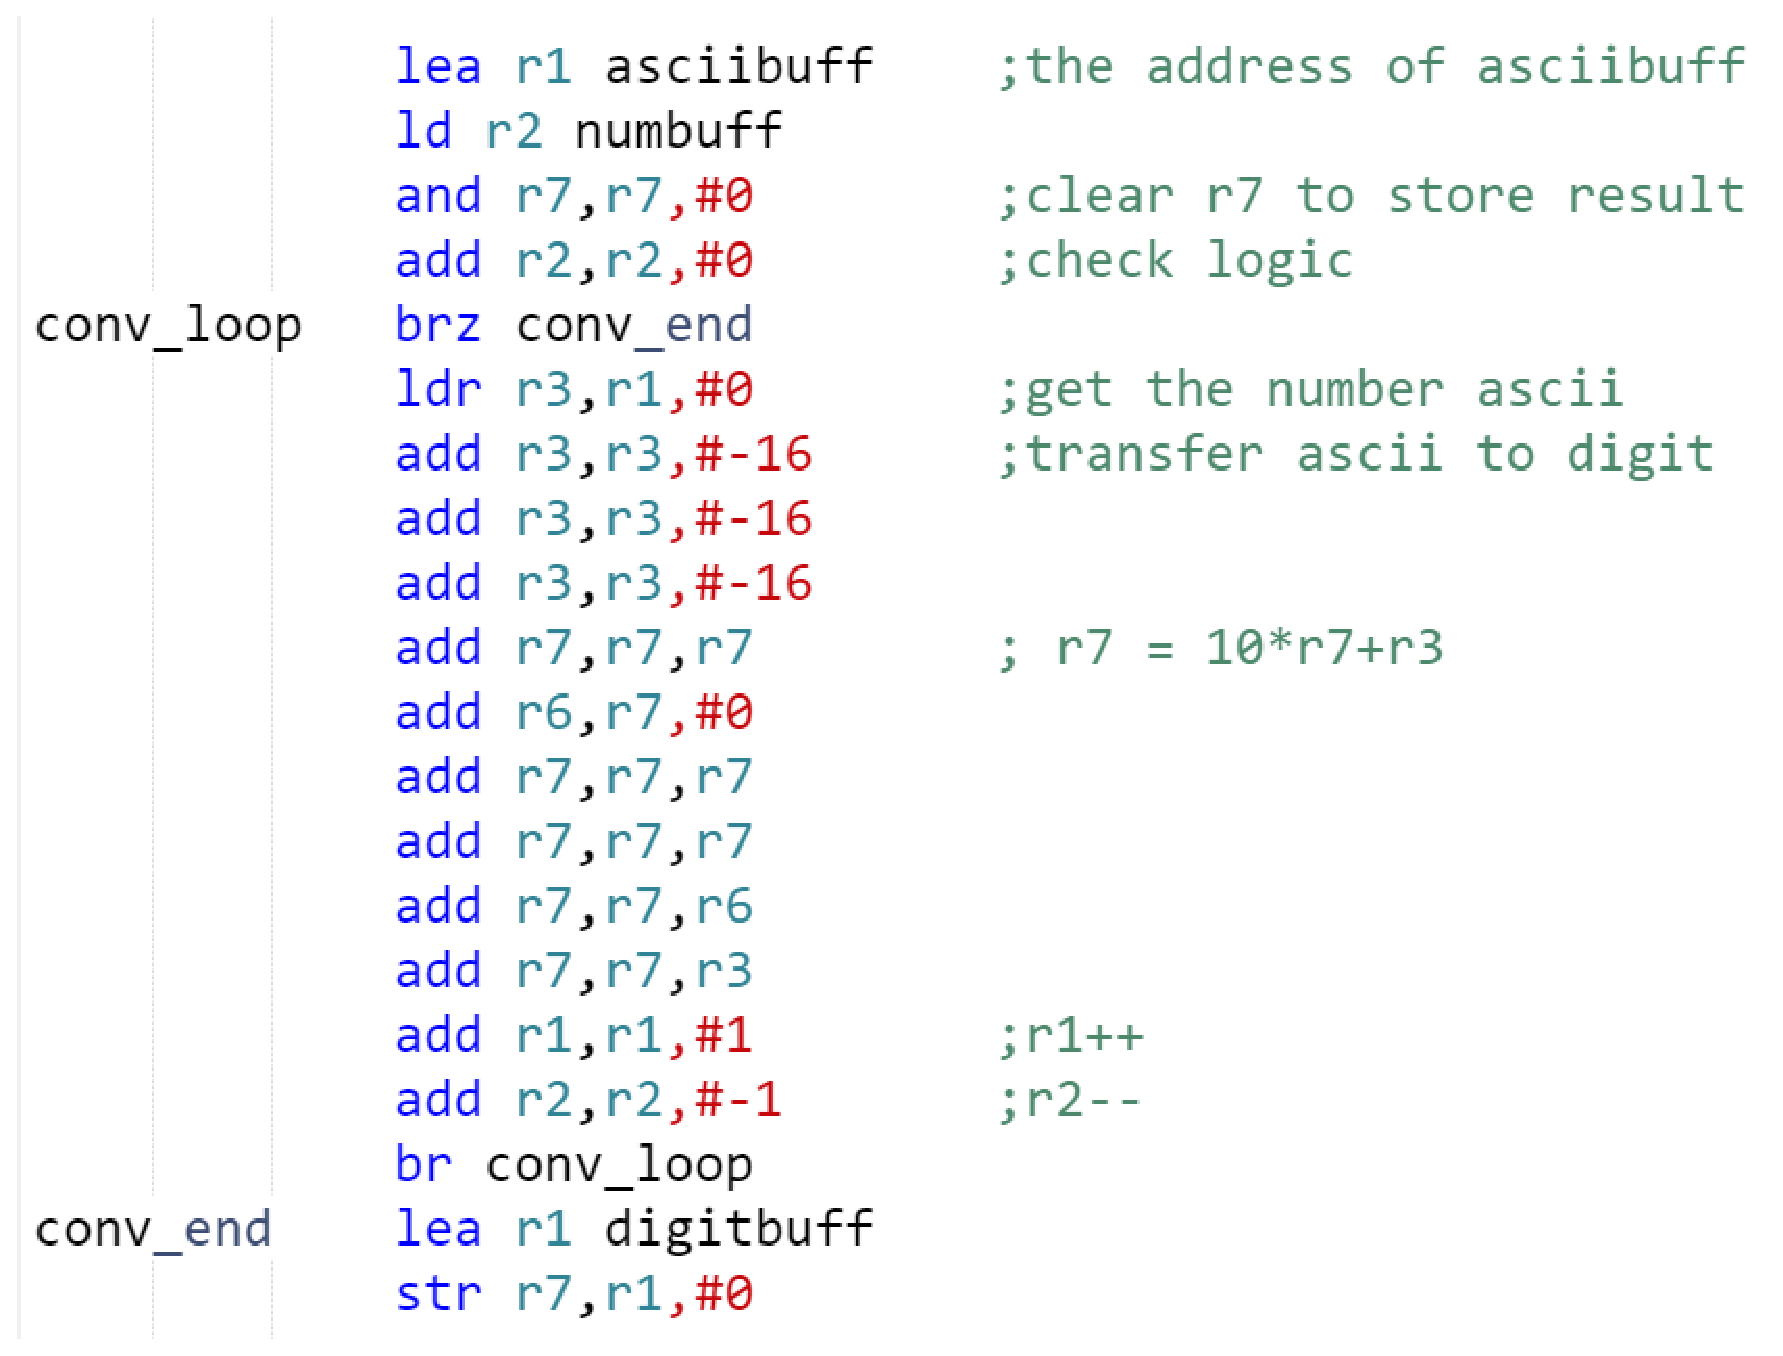
\includegraphics[width=0.7\textwidth]{fig1.eps}
		\caption{implement} %名字
	\end{figure}
	
	
	Fig 2 is the Lpop function

	\begin{figure}[htbp]
		\small
		\centering
		\includegraphics[width=0.7\textwidth]{fig2.eps}
		\caption{Lpop} %名字
	\end{figure}


	Fig 3 is the Lpush function
	
	\begin{figure}[htbp]
		\small
		\centering
		\includegraphics[width=0.7\textwidth]{fig3.eps}
		\caption{Lpush} %名字
	\end{figure}

\end{CJK*}
\end{document}





